\documentclass[varwidth=40cm]{standalone}
\usepackage{tikz}
\usetikzlibrary{patterns,decorations.pathreplacing}
\usepackage{style}

\begin{document}
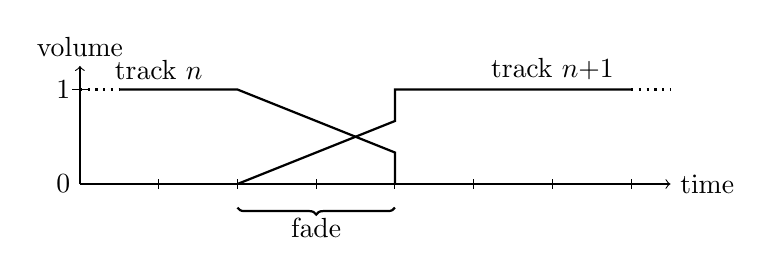
\begin{tikzpicture}[yscale=0.6]
  \draw[->] (0,0) -- (0,2.5);
  \draw (-0.1,2) -- (0.1,2);
  \draw (0,2) node[left]{1};
  \draw (0,0) node[left]{0};
  \draw[->] (0,0) -- (7.5,0);
  \foreach \x in {1,2,3,4,5,6,7} \draw (\x,-0.1) -- (\x,0.1);
  \draw (0,2.5) node[above]{volume};
  \draw (7.5,0) node[right]{time};
  \draw[thick,dotted] (0,2) -- (.5,2);
  \draw[thick] (.5,2) -- (2,2) -- (4,2/3) -- (4,0);
  \draw[thick] (2,0) -- (4,4/3) -- (4,2) -- (7,2);
  \draw[thick,dotted] (7,2) -- (7.5,2);
  \draw (1,2) node[above]{track $n$};
  \draw (6,2) node[above]{track $n{+}1$};
  \draw [thick, decoration={brace,mirror}, decorate] (2,-.5) -- (4,-.5) node [pos=0.5,below] {fade};
\end{tikzpicture}
\end{document}
